\documentclass[main.tex]{subfiles}

\begin{document}

\section{Theory and Model on the dynamics of squids}

\lipsum[1-2]

\begin{figure}[h]
    \centering
    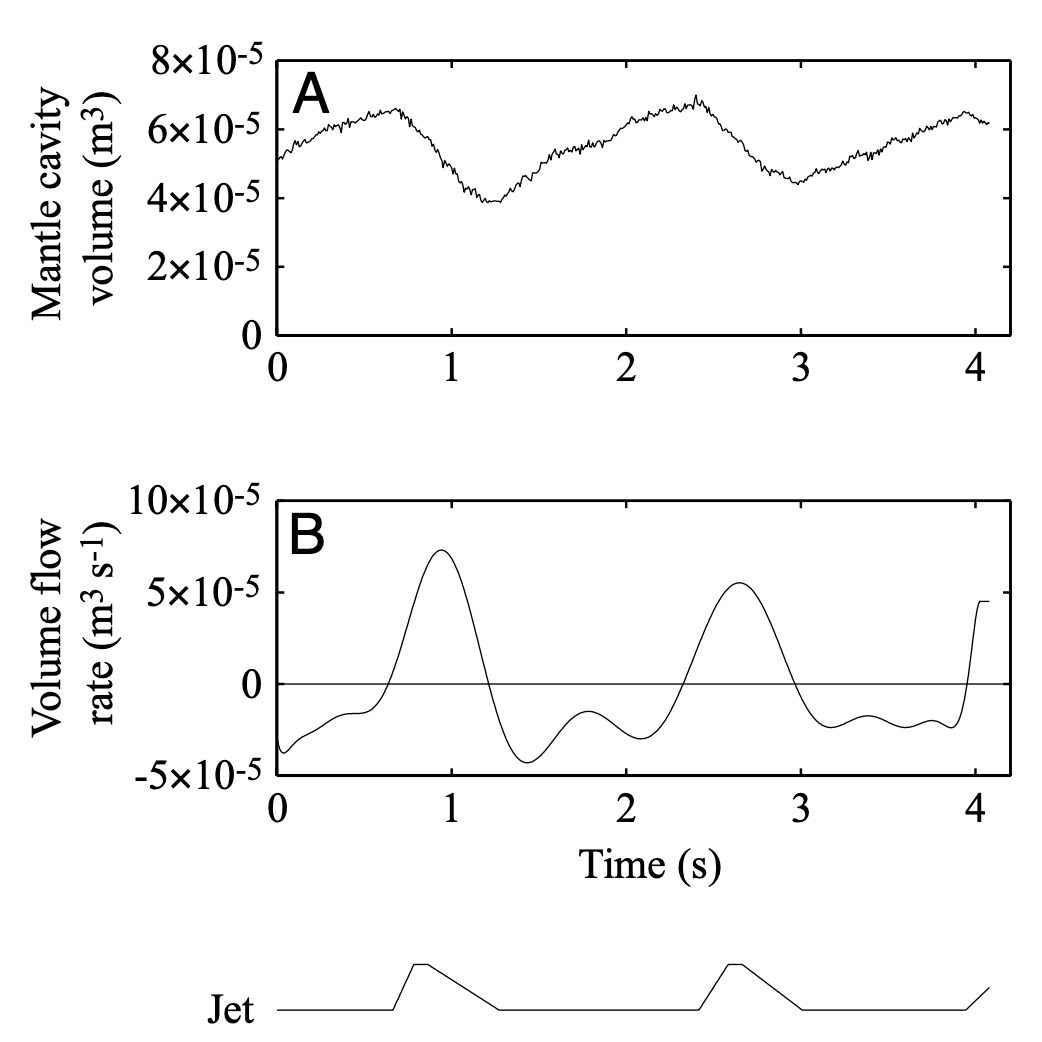
\includegraphics[width = 0.4\textwidth]{mantle_volume_s.png}
    \caption{Mantle cavity volume (A) and volume flow rate (B) for slow-swimming squid accompany by jet activity\cite{Anderson2000}}
\end{figure}

\begin{figure}[h]
    \centering
    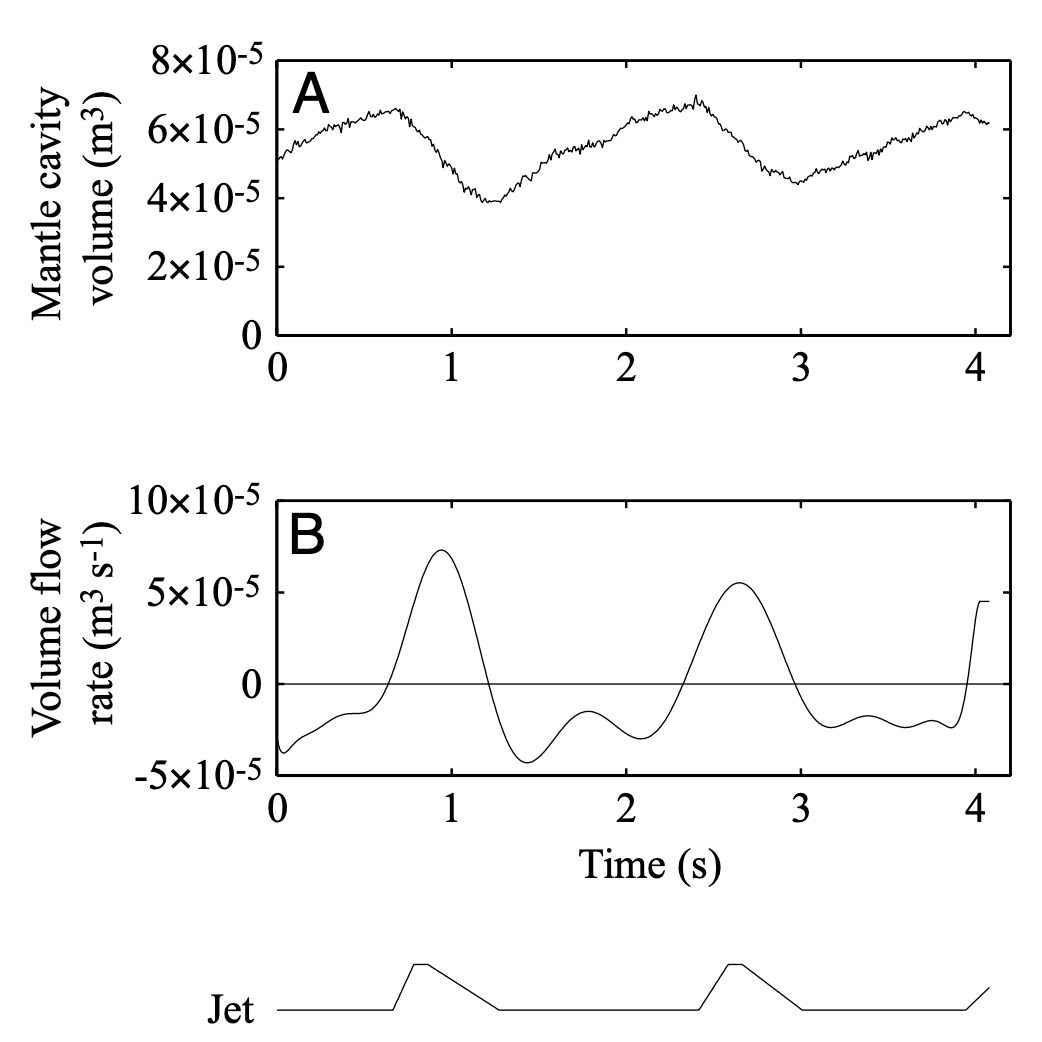
\includegraphics[width = 0.4\textwidth]{mantle_volume_s.png}
    \caption{Mantle cavity volume (A) and volume flow rate (B) for slow-swimming squid accompany by jet activity\cite{Anderson2000}}
\end{figure}

\begin{table}[h]
    \centering
    \begin{tabular}{|c|c|}
    \hline
    Parameters                    & Values         \\ \hline
    $D$ (diameter)                & $0.04m$        \\ \hline
    $L$ (length)                  & $0.2m$         \\ \hline
    $f$ (frequency)               & $60Hz$         \\ \hline
    $\rho$ (density of the fluid) & $998.2 kg/m^3$ \\ \hline
    \end{tabular}
    \caption{The parameters for thruster used in Robot}
\end{table}

\begin{table}[h]
    \centering
    \begin{tabular}{|c|c|}
    \hline
    Parameters                    & Values         \\ \hline
    $D$ (diameter)                & $0.04m$        \\ \hline
    $L$ (length)                  & $0.2m$         \\ \hline
    $f$ (frequency)               & $60Hz$         \\ \hline
    $\rho$ (density of the fluid) & $998.2 kg/m^3$ \\ \hline
    \end{tabular}
    \caption{The parameters for thruster used in Robot}
\end{table}

\section{Kinematics and dynamics of squids}

\lipsum[1-2]

\begin{figure}[h]
    \centering
    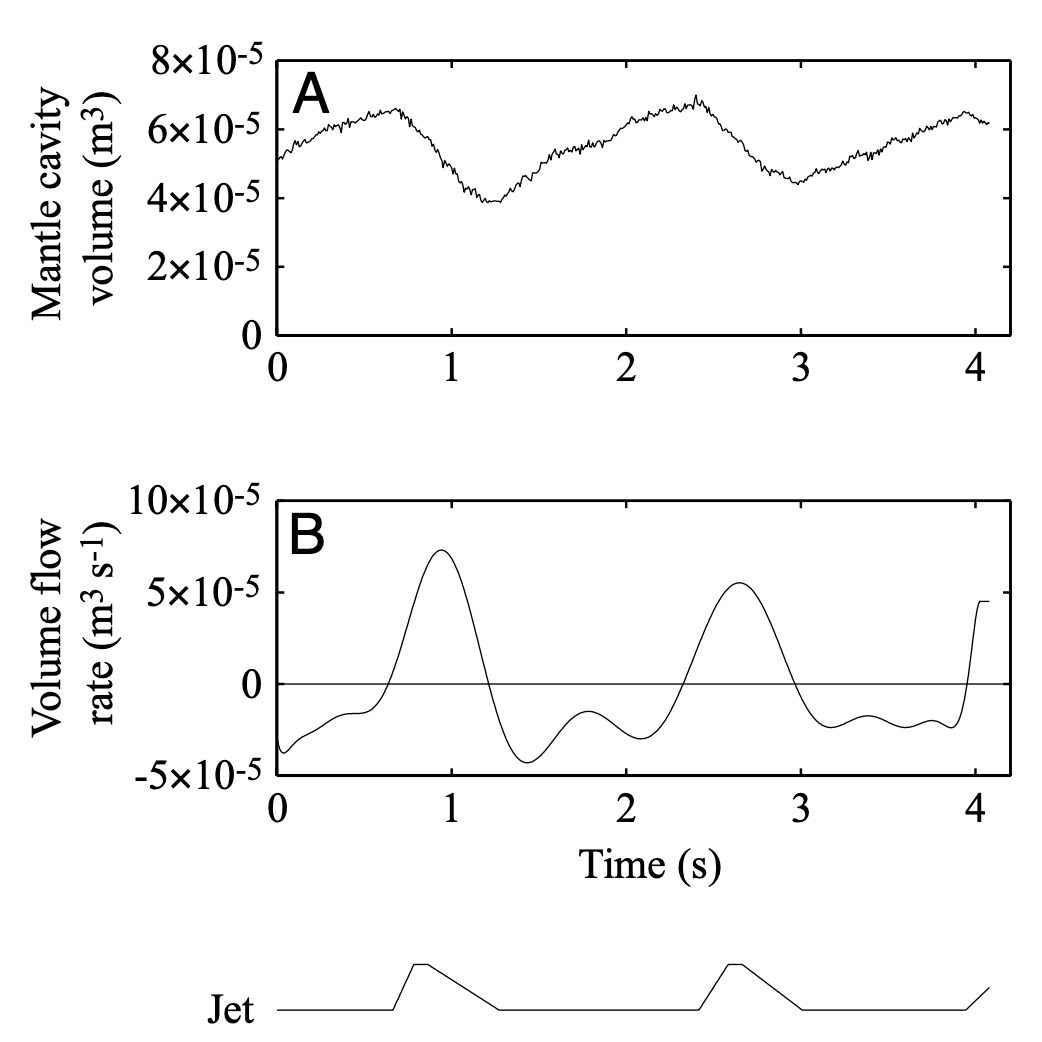
\includegraphics[width = 0.4\textwidth]{mantle_volume_s.png}
    \caption{Mantle cavity volume (A) and volume flow rate (B) for slow-swimming squid accompany by jet activity\cite{Anderson2000}}
\end{figure}

\subsection{Jet thrust and intramantle pressure}

\lipsum[1-2]
\begin{equation}
    \text{\sout{$V$}}_m(t) = \frac{\pi}{4}\int_0^{L_m}[D(\xi,t)]^2d\xi
\end{equation}
\lipsum[1]\cite{Anderson2000}. 

\subsubsection{Jet thrust and intramantle pressure}

\lipsum[1-2]

\begin{table}[h]
    \centering
    \begin{tabular}{|c|c|}
    \hline
    Parameters                    & Values         \\ \hline
    $D$ (diameter)                & $0.04m$        \\ \hline
    $L$ (length)                  & $0.2m$         \\ \hline
    $f$ (frequency)               & $60Hz$         \\ \hline
    $\rho$ (density of the fluid) & $998.2 kg/m^3$ \\ \hline
    \end{tabular}
    \caption{The parameters for thruster used in Robot}
\end{table}

\end{document}